\documentclass{article}
\usepackage[paperwidth=10.4cm,paperheight=8.4cm,margin=1mm]{geometry}
\usepackage[UTF8]{ctex}
\usepackage{amsmath,amssymb,bm}
\usepackage{tikz}
\usetikzlibrary{arrows.meta,calc}
\pagestyle{empty}
\begin{document}
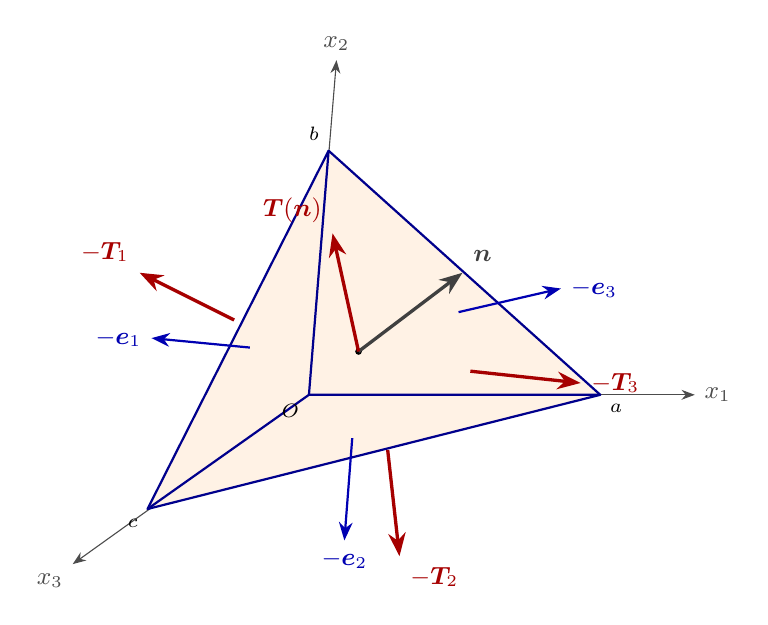
\begin{tikzpicture}[>=Stealth,font=\small,line join=round]
  % ===== 坐标轴与顶点 =====
  \coordinate (O) at (0,0);
  \coordinate (a) at (3.7,0);
  \coordinate (b) at (0.25,3.1);
  \coordinate (c) at (-2.05,-1.45);
  \draw[->,black!70] (O) -- (4.9,0) node[right] {$x_1$};
  \draw[->,black!70] (O) -- (0.35,4.25) node[above] {$x_2$};
  \draw[->,black!70] (O) -- (-3.0,-2.15) node[below left] {$x_3$};
  % ===== 四面体各面 =====
  \fill[blue!5]  (O) -- (a) -- (b) -- cycle;
  \fill[blue!8]  (O) -- (b) -- (c) -- cycle;
  \fill[blue!12] (O) -- (c) -- (a) -- cycle;
  \fill[orange!10] (a) -- (b) -- (c) -- cycle;
  \draw[blue!55!black,thick] (O) -- (a) (O) -- (b) (O) -- (c);
  \draw[blue!55!black,thick] (a) -- (b) -- (c) -- cycle;
  % ===== 顶点标注 =====
  \node[font=\scriptsize,below right] at (a) {$a$};
  \node[font=\scriptsize,above left] at (b) {$b$};
  \node[font=\scriptsize,below left] at (c) {$c$};
  \node[font=\scriptsize,below left] at (O) {$O$};
  % ===== 三个坐标面上的外法向 =====
  \draw[->,thick,blue!70!black] (-0.75,0.60) -- (-2.00,0.72) node[left] {$-\boldsymbol{e}_1$};
  \draw[->,thick,blue!70!black] (0.55,-0.55) -- (0.45,-1.85) node[below] {$-\boldsymbol{e}_2$};
  \draw[->,thick,blue!70!black] (1.90,1.05) -- (3.20,1.35) node[right] {$-\boldsymbol{e}_3$};
  % ===== 三个坐标面上的应力矢量 =====
  \draw[->,very thick,red!65!black] (-0.95,0.95) -- (-2.15,1.55) node[above left] {$-\boldsymbol{T}_1$};
  \draw[->,very thick,red!65!black] (1.00,-0.70) -- (1.15,-2.05) node[below right] {$-\boldsymbol{T}_2$};
  \draw[->,very thick,red!65!black] (2.05,0.30) -- (3.45,0.15) node[right] {$-\boldsymbol{T}_3$};
  % ===== 斜面上的法向与应力 =====
  \coordinate (M) at (0.63,0.55);
  \fill (M) circle (1.2pt);
  \draw[->,very thick,black!75] (M) -- (1.95,1.55) node[above right] {$\boldsymbol{n}$};
  \draw[->,very thick,red!65!black] (M) -- (0.30,2.05) node[above left] {$\boldsymbol{T}(\boldsymbol{n})$};
\end{tikzpicture}
\end{document}
